\chapter{Evaluation}

\chapterintro{
  This chapter contains results and discussions on the evaluation of tests run on the proposed solution.
}

\section{Introduction}
We carried out a number of tests which aim to prove the solution be better than currently available, especially in terms of:
\begin{enumerate}
  \item deployment cost
  \item cost of providing given Quality-of-Service
  \item deployment time
\end{enumerate}

\section{Cost of service deployment}
\subsection*{Description}
The aim of this test case is to test the primary use case of the proposed solution -- deployment of a service with the emphasis of client's \textbf{cost}. It should show that the platform chooses the best mapping between the stacks and cloud providers so that the client's pays the \textbf{lowest} possible price.

\subsection*{Preconditions}
Service specification (\ref{lst:service-spec-test-cost}) forms an input to the application. Its elements are different software stacks that are parts of the whole service. Each cloud provider has its own price for a given software stack which is shown in table \ref{tbl:test-service-deployment-cost}. Diagram \ref{eval:deployment-cost-physical-nodes} illustrates the simplified environment setup.

\begin{table}
  \centering
  \begin{tabular}{ | c | c | c | c | }
    \hline                        
    & CP-1 & CP-2 & CP-3 \\
    \hline
    java      & 150 & 120 & 180 \\
    ruby      & 220 & 290 & 250 \\
    postgres  & 320 & 240 & 290 \\
    python    & 200 & 260 & 180 \\
    amqp      & 330 & 390 & 285 \\
    \hline  
  \end{tabular}
  \caption{Price for a stack in the given cloud provider}
  \label{tbl:test-service-deployment-cost}
\end{table}

\begin{figure}[!ht]
  \begin{center}
    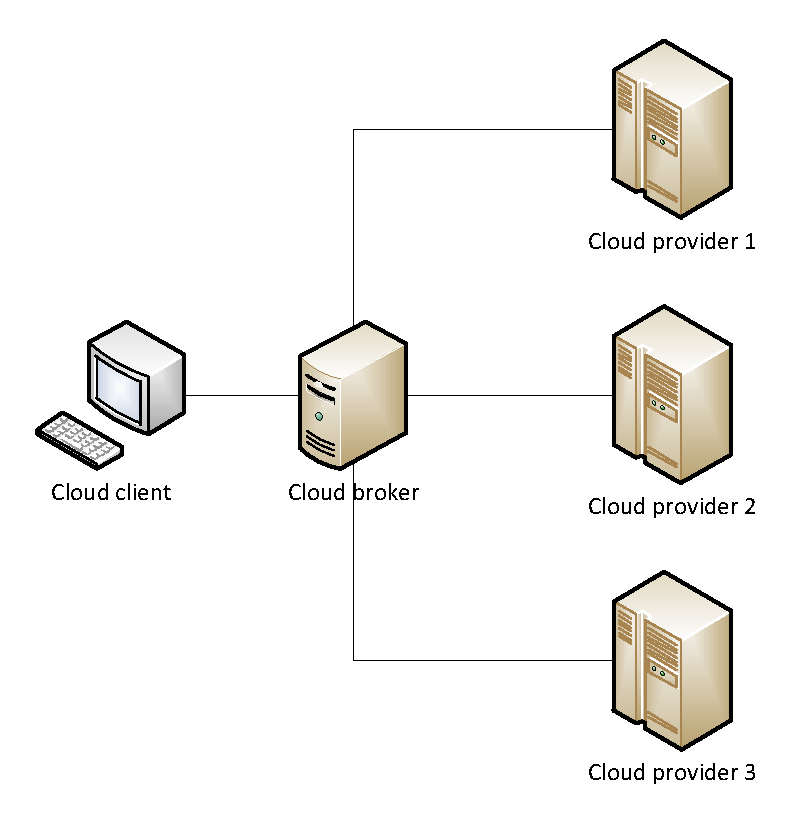
\includegraphics[width=0.6\textwidth]{chapter-7/deployment-cost-physical-nodes}
  \end{center}
  \caption{Deployment cost: environment configuration}
  \label{eval:deployment-cost-physical-nodes}
\end{figure}


\subsection*{Results}
Table \ref{tbl:test-service-deployment-cost-mapping} shows obtained mapping between stacks and cloud providers. Taking into account this result, figure \ref{ch7:service-deployment-cost} shows comparison of cost the client would have to pay with and without such a mapping.

\begin{table}
  \centering
  \begin{tabular}{ | c | c | c | c | }
    \hline                        
    & CP-1 & CP-2 & CP-3 \\
    \hline
    java      & & x & \\
    ruby      & x & & \\
    postgres  & & x & \\
    python    & & & x \\
    amqp      & & & x \\
    \hline  
  \end{tabular}
  \caption{Chosen cloud providers for the given stack}
  \label{tbl:test-service-deployment-cost-mapping}
\end{table}

\begin{figure}[!ht]
  \begin{center}
    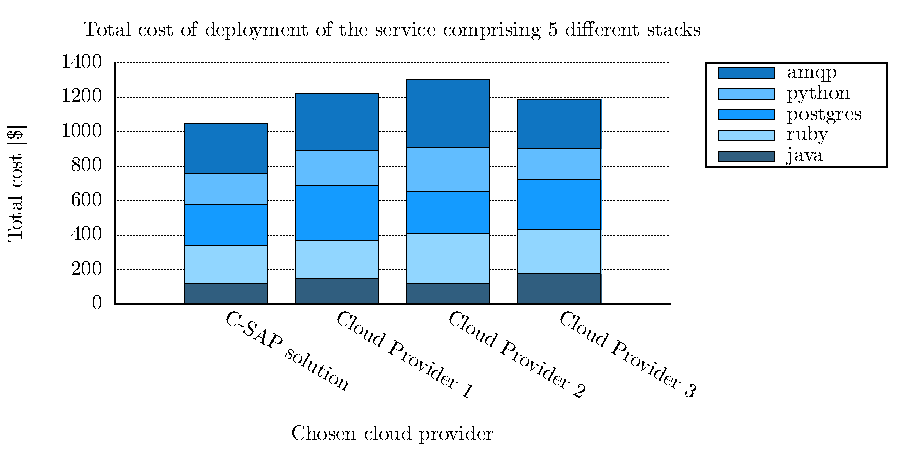
\includegraphics{chapter-7/case-study-service-deployment-reduced-client-costs}
  \end{center}
  \caption{Comparison of the deployment cost when the service is deployed only on a selected cloud provider or a combination of cloud providers selected by Cloud-SAP}
  \label{ch7:service-deployment-cost}
\end{figure}

\subsection*{Conclusion}

\section{Auto-scaling -- single-provider based}
\subsection*{Description}
\subsection*{Preconditions}
\begin{figure}[!ht]
  \begin{center}
    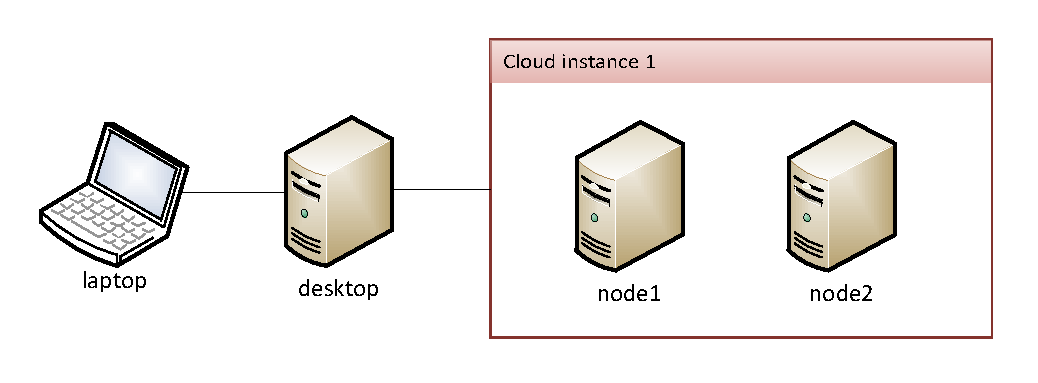
\includegraphics[width=0.8\textwidth]{chapter-7/auto-scaling-1cp-physical-nodes}
  \end{center}
  \caption{Auto-scaling - single-provider based: environment configuration}
  \label{eval:auto-scaling-1cp-physical-nodes}
\end{figure}

\subsection*{Results}
\subsection*{Conclusion}

\section{Auto-scaling -- multiple-provider based}
\subsection*{Description}
\subsection*{Preconditions}
\begin{figure}[!ht]
  \begin{center}
    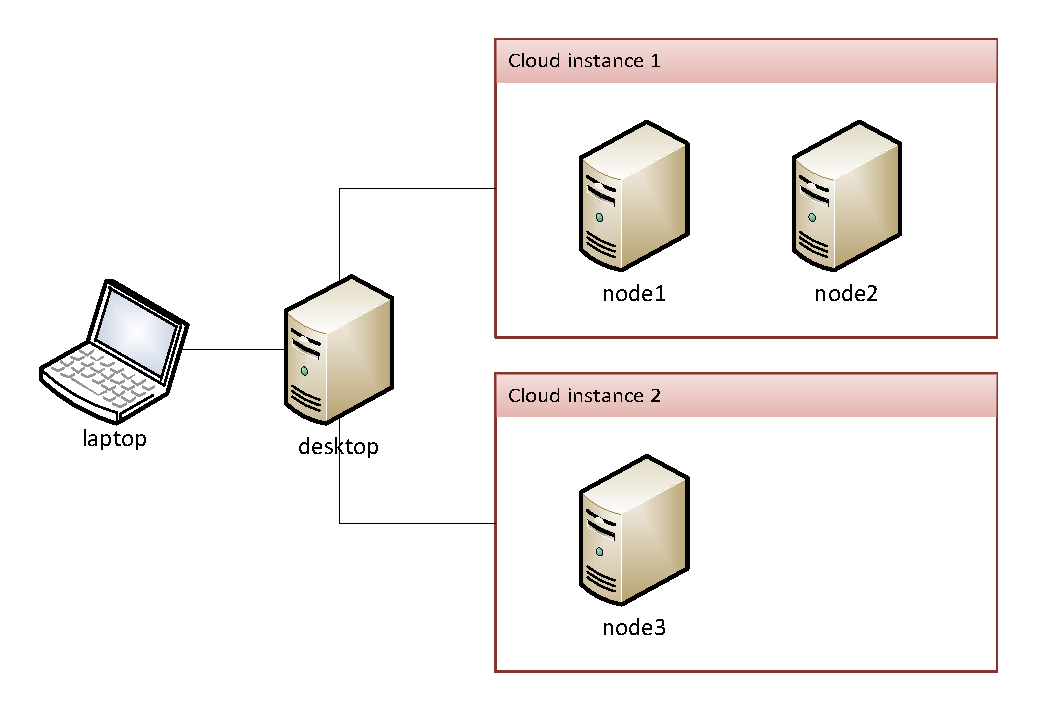
\includegraphics[width=0.8\textwidth]{chapter-7/auto-scaling-2cp-physical-nodes}
  \end{center}
  \caption{Auto-scaling - multiple-provider based: environment configuration}
  \label{eval:auto-scaling-1cp-physical-nodes}
\end{figure}

\subsection*{Results}
\subsection*{Conclusion}

\section{Deployment time -- solution comparison}
\subsection*{Description}
In this test we want to compare our solution to one of those available at the market which use \emph{OpenNebula} as an underlying tool for managing resources of a data center and \emph{OpenVZ} as a hypervisor in terms of \textbf{deployment time}, one of the most important factors of products whose main purpose is to scale applications.
\emph{Carina} \cite{Carina} can be considered a perfect match of a solution for such a comparison and tests are ran against it.

This test involves the steps of
  \begin{inparaenum}[i)]
    \item instantiating one of the tested product, i.e. Cloud-SAP or Carina,
    \item ordering the deployment of a service whose specification is shown in listing \ref{lst:service-spec-test-deployment-time},
    \item measuring the time needed to set up the environment of the service.
  \end{inparaenum}

\subsection*{Preconditions}
It is assumed that \emph{Cloud-SAP} and \emph{Carina} according with \emph{OpenVZ} as an underlying virtualization technology are correctly installed and configured.
Each test case must be run in an isolation so before performing any test all virtual machines present at the deployment node are removed.
\subsubsection{OpenNebula configuration}
To ensure objectivity in tests, OpenNebula was configured in both products in the same way. One of the key factors that could influence the deployment time is the configuration of scheduler. Its parameters are shown in the listing \ref{lst:one-scheduler-config}.
\lstinputlisting[caption=OpenNebula scheduler configuration, label=lst:one-scheduler-config]{deployment-time-test-sched-config}
\subsubsection{Service description}
The service comprises a simple java enterprise application, deployed in a master-slave configuration with one VM set as a load balancer and other nodes that serve as workers, which uses Tomcat as a web container.

The description of a service expressed in Carina format can be found in listing \ref{lst:carina-config}.

- TODO dodać konfigurację każdej z maszyn wirtualnych 

\subsubsection{Hardware configuration}
All virtual machines were deployed on one node which had 3G RAM, AMD Athlon\texttrademark 64 X2 Dual Core Processor with each core of 2000 MHz frequency and a hard drive with a capacity of 160 GB. Diagram presents the physical configuration of nodes.

+ fizycznych

\begin{figure}[!ht]
  \begin{center}
    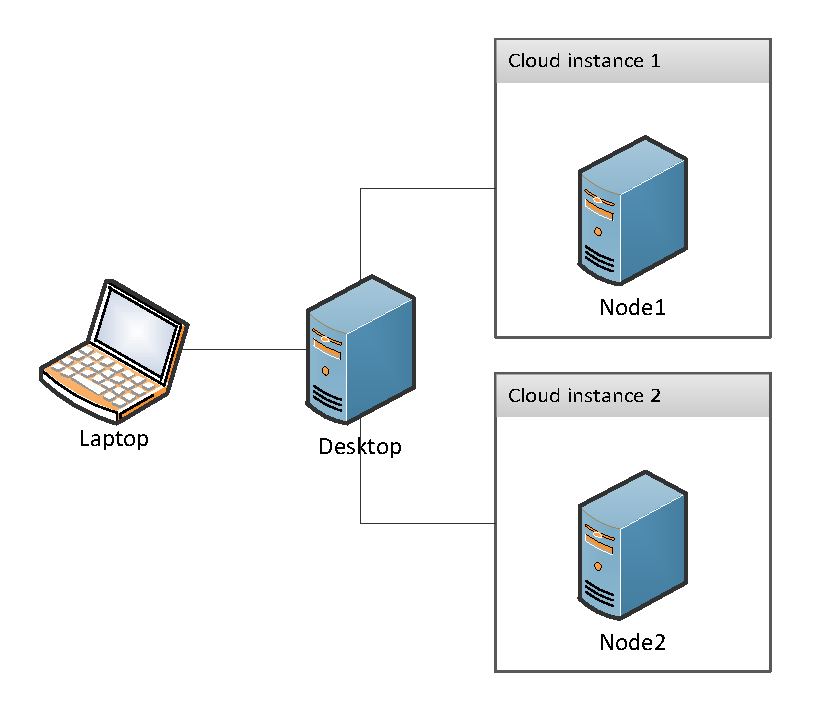
\includegraphics[width=0.6\textwidth]{chapter-7/deployment-time-physical-nodes}
  \end{center}
  \caption{Deployment time - solution comparison: physical environment setup}
  \label{eval:deployment-time-physical-nodes}
\end{figure}

\subsubsection{Environment configuration}
Deployment diagram for \emph{Carina} implementation is shown in figure \ref{ch7:deployment-time-test-deployment-time-carina-deployment-diagram} and for \emph{Cloud-SAP} in figure \ref{ch7:deployment-time-test-cloud-sap-deployment-diagram}.

\begin{figure}[!ht]
  \begin{center}
    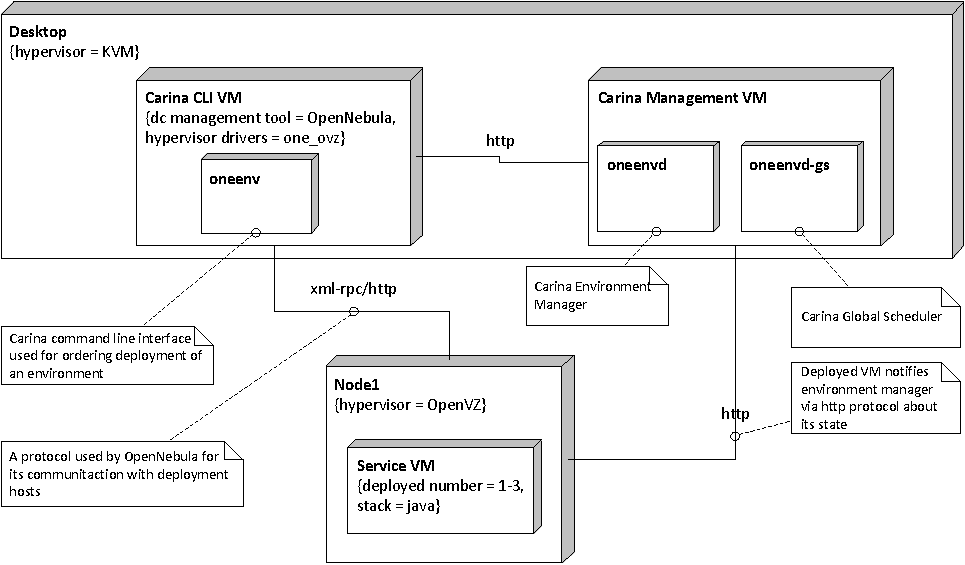
\includegraphics{chapter-7/deployment-time-carina-deployment-diagram}
  \end{center}
  \caption{Deployment diagram of \emph{Carina}}
  \label{ch7:deployment-time-test-deployment-time-carina-deployment-diagram}
\end{figure}

\begin{figure}[!ht]
  \begin{center}
    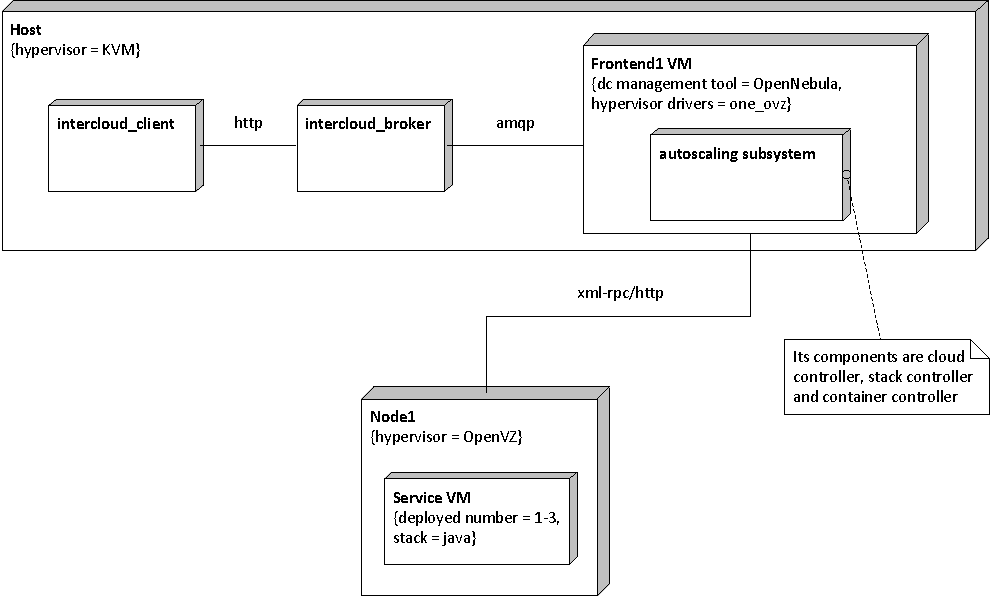
\includegraphics{chapter-7/deployment-time-test-cloud-sap-deployment-diagram}
  \end{center}
  \caption{Deployment diagram of \emph{Cloud-SAP}}
  \label{ch7:deployment-time-test-cloud-sap-deployment-diagram}
\end{figure}

\subsection*{Results}
Obtained results are shown in table \ref{tbl:test-service-deployment-time} and in figure \ref{ch7:deployment-time-test}. For a given number of instances we ordered deploying a service 10 times and the values shown in those figures are an average of these runs.

\begin{table}
  \centering
  \begin{tabular}{ c  c  c }
    \hline
    & \multicolumn{2}{c}{Solution} \\
    \cline{2-3}
    Instance no & Cloud-SAP & Carina \\
    \hline
    2 & 198.0 & 158.7s \\
    3 & 261.72 & 208.1s \\
    4 & 294.38 & 230.6s \\
    \hline
  \end{tabular}
  \caption{Average deployment time for the service with the various number of VMs used for the whole environment}
  \label{tbl:test-service-deployment-time}
\end{table}

\begin{figure}[!ht]
  \begin{center}
    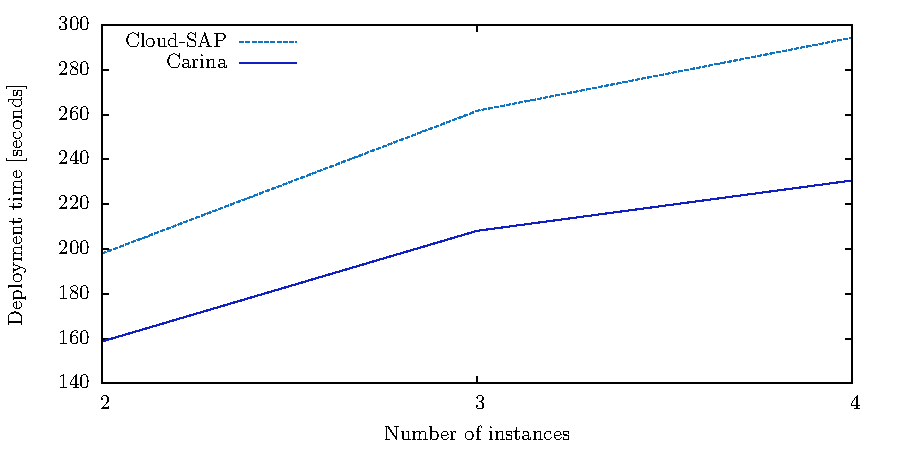
\includegraphics{chapter-7/deployment-time-test}
  \end{center}
  \caption{Average deployment time for two competing products when the variable is the number of instances of VMs}
  \label{ch7:deployment-time-test}
\end{figure}

\subsection*{Conclusion}


\section{Deployment time -- hypervisor comparison}
\subsection*{Description}
\subsection*{Preconditions}
\subsection*{Results}
\subsection*{Conclusion}

